%============================================================
% TEACHER GENERATION
%============================================================

\section{Teacher Generation}

%------------------------------------------------------------
% TEACHER GENERATION - SLIDE 1
%------------------------------------------------------------

\begin{frame}
    \frametitle{Teacher Generation}

    \small

    \begin{block}{Mục tiêu}
        Sử dụng teacher model để sinh dữ liệu
        \textbf{Chain-of-Thought (CoT)} từ đáp án và
        luồng suy luận mẫu.
    \end{block}

    \vspace{0.3cm}

    \begin{center}
    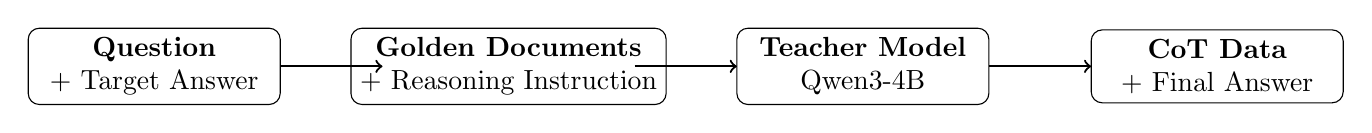
\begin{tikzpicture}[
        every node/.style={align=center},
        box/.style={
            draw,
            rounded corners,
            minimum width=3.2cm,
            minimum height=0.9cm
        },
        arrow/.style={
            ->,
            thick
        }
    ]

        \node[box] at (0,0)
        {\textbf{Question}\\
        + Target Answer};

        \node[box] at (4.5,0)
        {\textbf{Golden Documents}\\
        + Reasoning Instruction};

        \node[box] at (9,0)
        {\textbf{Teacher Model}\\
        Qwen3-4B};

        \node[box] at (13.5,0)
        {\textbf{CoT Data}\\
        + Final Answer};

        \draw[arrow] (1.6,0) -- (2.9,0);
        \draw[arrow] (6.1,0) -- (7.4,0);
        \draw[arrow] (10.6,0) -- (11.9,0);

    \end{tikzpicture}
    \end{center}

    \vspace{0.35cm}

    \begin{block}{Teacher Model}
        \centering
        \textbf{Qwen3-4B}
    \end{block}

    \vspace{0.15cm}

    \begin{itemize}
        \item Không cần model quá lớn vì teacher chỉ dùng để
        sinh CoT từ đáp án và reasoning structure có sẵn.

        \item Target answer và reasoning instruction được dùng
        làm supervision cho quá trình teacher generation.

        \item Output gồm reasoning process và final answer.
    \end{itemize}

\end{frame}


%------------------------------------------------------------
% TEACHER GENERATION - SLIDE 2
%------------------------------------------------------------

\begin{frame}[t]
    \frametitle{Teacher Generation: Teacher Prompt (1/3)}

    \scriptsize

    \textbf{You are a reasoning teacher generating high-quality reasoning
    data for a retrieval-augmented language model.}

    \vspace{0.1cm}

    Your task is to solve the question below by reasoning over the
    provided documents.

    \vspace{0.08cm}

    The target answer is provided intentionally as supervision for
    this teacher-generation process.

    \vspace{0.1cm}

    \textbf{IMPORTANT:}

    \begin{itemize}
        \item You are given the final answer as a target.
        \item Reconstruct a natural reasoning process that leads to
        that answer.
        \item Do NOT simply explain the answer directly.
        \item Start from the original question.
        \item Determine what information is required.
        \item Identify the relevant evidence.
        \item Connect intermediate facts when the question requires
        multi-hop reasoning.
        \item Every factual claim should be grounded in the provided
        documents whenever possible.
        \item When referring to a document, ALWAYS use its exact Title.
        \item NEVER refer to documents as ``Document 1'', ``Document 2'',
        etc.
        \item Do not mention that you were given the target answer.
        \item Do not mention internal dataset annotations.
        \item Do not mention document labels such as
        ``[GOLDEN DOCUMENT]'' or ``[END DOCUMENT]'' in the reasoning.
        \item Do not mention this instruction.
        \item Do not introduce information that is not supported by
        the provided documents.
    \end{itemize}

    \vspace{0.03cm}

    The final answer should be concise and appear at the end in
    exactly this form:

    \begin{center}
        \texttt{<answer>}\\
        \texttt{short answer}\\
        \texttt{</answer>}
    \end{center}

\end{frame}


%------------------------------------------------------------
% TEACHER GENERATION - SLIDE 3
%------------------------------------------------------------

\begin{frame}[t]
    \frametitle{Teacher Generation: Teacher Prompt (2/3)}

    \scriptsize

    \textbf{QUESTION}

    \vspace{0.04cm}

    What watercourse is the river on which the Lostock Dam is located
    the mouth of?

    \vspace{0.1cm}

    \textbf{TARGET ANSWER}

    \vspace{0.03cm}

    Hunter River

    \vspace{0.1cm}

    \textbf{GOLDEN DOCUMENTS}

    \vspace{0.03cm}

    The following documents provide the evidence needed
    to solve the question.

    \vspace{0.06cm}

    \textbf{[GOLDEN DOCUMENT]}

    \textbf{Title: Lostock Dam}

    Lostock Dam is a minor rockfill and clay core embankment dam with
    a concrete lined, flip bucket spillway across the Paterson River
    upstream of the village of East Gresford in the Hunter region of
    New South Wales, Australia. The dam's purpose includes flood
    mitigation, irrigation, water supply and conservation. Mini
    hydro-power facilities were retrofitted in 2010. The impounded
    reservoir is also called Lostock Dam.

    \vspace{0.03cm}

    \textbf{[END DOCUMENT]}

    \vspace{0.06cm}

    \textbf{[GOLDEN DOCUMENT]}

    \textbf{Title: Paterson River}

    Paterson River, a perennial river that is part of the Hunter River
    catchment, is located in the Hunter and Mid North Coast regions of
    New South Wales, Australia.

    \vspace{0.03cm}

    \textbf{[END DOCUMENT]}

\end{frame}


%------------------------------------------------------------
% TEACHER GENERATION - SLIDE 4
%------------------------------------------------------------

\begin{frame}[t]
    \frametitle{Teacher Generation: Teacher Prompt (3/3)}

    \scriptsize

    \textbf{REASONING INSTRUCTION}

    \vspace{0.04cm}

    Use the following reasoning structure to solve the main question.
    The information below is provided as teacher supervision.
    Reconstruct a natural reasoning process from it rather than
    copying it verbatim.

    \vspace{0.06cm}

    \textbf{Main question:} What watercourse is the river on which the
    Lostock Dam is located the mouth of?

    \vspace{0.05cm}

    \textbf{Reasoning steps:}

    \textbf{Step 1:}

    Sub-question: Lostock Dam >> located on terrain feature

    Intermediate answer: Paterson River

    Supporting document: Lostock Dam

    \vspace{0.05cm}

    \textbf{Step 2:}

    Sub-question: \#1 >> mouth of the watercourse

    Intermediate answer: Hunter River

    Supporting document: Paterson River

    \vspace{0.05cm}

    \textbf{Final answer:} Hunter River

    \vspace{0.08cm}

    \textbf{TASK}

    \vspace{0.04cm}

    Reason through the question step by step.

    Use the provided reasoning instruction to guide the reasoning.

    Start from the original question.

    Determine what information is required.

    Identify the relevant evidence in the provided documents.

    Follow the necessary information dependencies between
    intermediate facts.

    For multi-hop questions, clearly connect the intermediate
    answers so that the final answer follows naturally from them.

    When referring to evidence, identify the source using its exact
    document Title.

    Do not refer to documents using positional names such as
    ``Document 1'' or ``Document 2''.

    Do not mention that the answer was provided as supervision.
    Do not mention the dataset, annotations, or these instructions
    in the reasoning.

    Write a natural, coherent reasoning process.

    At the end, provide the concise final answer using exactly:

    \begin{center}
        \texttt{<answer>}\\
        \texttt{short answer}\\
        \texttt{</answer>}
    \end{center}

\end{frame}